\documentclass[conference]{IEEEtran}
\usepackage[spanish]{babel}
\usepackage[latin1]{inputenc}
\usepackage{blindtext, graphicx}
\usepackage{subfigure}
\usepackage{mdwmath}
\usepackage{mdwtab}
\usepackage{subfig}
\usepackage{amsmath}

\begin{document}
\title{ Aplicaci\'on del m\'etodo de Canny para la detecci\'on de bordes de una imagen digital }
\author{\IEEEauthorblockN{Walter Alejandro Moreno Ram\'irez}
\IEEEauthorblockA{Departamento de Estudios Multidisciplinarios\\
Universidad de Guanajuato\\
Yuriria, Guanajuato\\
Correo: wa.morenoramirez@ugto.mx}}

\maketitle
\renewcommand\abstractname{Abstract}
\begin{abstract}
This article describes what are the edges of an image, as they can be detected by Canny method. Its advantages and applications will also be stated. \\\\
\end{abstract}

\begin{IEEEkeywords}
Pixel, p\'ixeles, convoluci\'on, canny, smoothing, suavizado, gradiente, segmentaci\'on ,primera derivada, funci\'on, C++, OpenCV, ventana, m\'ascara, vecindario.
\end{IEEEkeywords}

\IEEEpeerreviewmaketitle
\section{Introducci\'on}
Existen varios algoritmos para detectar los bordes de los objetos en una imagen digital, entre ellos, las matrices de convoluci\'on son una muy buena t\'ecnica para la detecci\'on de bordes; donde se puede utilizar una matriz de convoluci\'on ya sea de primera o segunda derivada. Ya que dichas matrices se basan en la raz\'on de cambio o un cambio muy dr\'astico en los tonos de grises en los vecinos de un pixel central. \\\\
Para esta pr\'actica se utiliza el algoritmo de Canny para la detecci\'on de bordes. Fue desarrollado por John F. Canny en 1986 y se basa en una secuencia de t\'ecnicas que se aplican sobre una imagen. Este algoritmo tiene como objetivo principal satisfacer tres criterios principales:\\
\begin{itemize}
	\item \textbf{Baja tasa de error}: esto se refiere a una buena detecci\'on de los bordes existentes.
	\item \textbf{Buena localizaci\'on}: la distancia entre los pixeles de borde detectados y los pixeles de borde reales es reducida.
	\item \textbf{Respuesta m\'inima}: s\'olo un detector responde por borde.\\
\end{itemize}

Podemos visualizar dicho algoritmo como una cadena, donde el resultado de cada t\'ecnica pasa al siguiente eslab\'on, teniendo como resultado final una imagen con los bordes de los objetos presentes en la imagen de entrada.\\

El algoritmo de Canny para la detecci\'on de bordes se basa en cuatro t\'ecnicas o componentes:\\
\begin{itemize}
	\item \textbf{Suavizado}: la finalidad de suavizar la imagen es la de atenuar el ruido presente en la imagen. Esto se logra ya sea con una matriz de mediana, promedio o con una matriz gaussiana.\\
	\item \textbf{Gradiente y angulos}: una vez la imagen fue suavizada, se procede a obtener el gradiente y el \'angulo para cada pixel de la imagen.\\
	\item \textbf{Supresi\'on de no-m\'aximos}: se eliminan los p\'ixeles cuyo gradiente sea de menor longitud con respecto al de sus vecinos que se encuentren en la direcci\'on positiva y negativa del \'angulo central de una ventana de 3x3.\\
	\item \textbf{Hist\'eresis}: este \'ultimo paso ubica los p\'ixeles en tres secciones delimitadas por dos umbrales. Estas secciones categorizan a los p\'ixeles como ``d\'ebiles'',  ``medios'' o ``fuertes'' y lo que hace es formar una continuidad entre los p\'ixeles ``fuertes'' ya que representan los bordes de la imagen.\\
\end{itemize}

\section{Metodolog\'ia}
\textbf{\\ Suavizado de la imagen:\\\\}
Como primer paso del algoritmo se suaviza la imagen. Debido a que los bordes de una imagen pueden ser f\'acilmente confundidos por ruido, al suavizar la imagen se desea atenuar el ruido para poder prevenir la detecci\'on de falsos bordes.\\
Para realizar este paso se utiliz\'o un filtro gaussiano de 5x5 con $\sigma = 1,5$, lo que da como resultado la matriz mostrada en la Ecuaci\'on (1). \\
\begin{equation}
B =
	\begin{bmatrix}
	 2 & 4 & 5 & 4 & 2 \\
	 4 & 9 & 12 & 9 & 4\\
	 5 & 12 & 15 & 12 & 5 \\
	 2 & 4 & 5 & 4 & 2 \\
	 4 & 9 & 12 & 9 & 4\\
	\end{bmatrix}
\end{equation}
Una vez se definio el filtro para el suavizado y, dada una imagen $A$ de entrada, se realiza la convoluci\'on entre dicho filtro y la imagen.
\begin{equation}
	imageOut = A \ast B
\end{equation}
De acuerdo a la Ecuaci\'on (2), nos muestra que el resultado de la convoluci\'on es una imagen que se pasa al siguiente eslab\'on de la cadena que es el algoritmo de Canny.\\
\textbf{\\ Obtener bordes:\\\\}
La siguiente fase del algoritmo es la detecci\'on de los bordes de la imagen, para ello se utiliz\'o un kernel, mas espec\'ificamente, los kernel de Sobel para detectar la raz\'on de cambio tanto en el eje $x$ como en el eje $y$ de la imagen. Por lo anterior, los kernel o filtros de Sobel son de primera derivada, dichos kernel se muestran en la Ecuaci\'on (3).\\\\
\begin{equation}
G_x = 
	\begin{bmatrix}
		-1 & 0 & 1 \\
		-2 & 0 & 2 \\
		-1 & 0 & 1 \\
	\end{bmatrix}
G_y = 
	\begin{bmatrix}
		-1 & -2 & -1 \\
		0 & 0 & 0 \\
		1 & 2 & 1 \\
	\end{bmatrix}
\end{equation}

Para obtener los bordes es necesario realizar una convoluci\'on entre cada kernel con la imagen suavizada, lo que da como resultado el gradiente de la imagen en ambas direcciones, $x$ y $y$.\\
Para unificar estos bordes y, de acuerdo a la Ecuaci\'on (4), se obtiene la magnitud del gradiente de la imagen.\\\\
\begin{equation}
	G = \sqrt{G_{x}^2 + G_{y}^2}
\end{equation}
Tambi\'en se obtiene el \'angulo de acuerdo a la Ecuaci\'on (5).
\begin{equation}
	\theta =  \tan^{-1}\left(\frac{G_y}{G_x}\right)
\end{equation}

Ya que el resultado de la funci\'on $atan2$, que esta incluida en la librer\'ia $cmath$ para C++, arroja un resultado en radianes, es necesario hacer una conversi\'on de radianes a grados multiplicando por $180$ y dividiendo entre $\pi$. Despu\'es se discretiza el \'angulo resultante para cada pixel, en un multiplo de $\pi /4$. Para dicha discretizaci\'on los \'angulos se tomar\'an de acuerdo a la Ecuaci\'on (6).

\begin{equation}
    \theta(p) = \left\{
       \begin{array}{ll}
	 0^{\circ} \leftarrow 157.5 \leq p \leq 22.5   \\
	45^{\circ} \leftarrow 22.5 \leq p < 67.5 \\
	90^{\circ} \leftarrow 67.5 \leq p < 112.5 \\
   135^{\circ} \leftarrow 112.5 \leq p < 157.5 \\
       \end{array}
    \right.
\end{equation}

\textbf{\\ Supresi\'on de no-m\'aximos:\\\\}
Una vez se hizo la discretizaci\'on de las direcciones del gradiente, el siguiente paso del algoritmo es eliminar los p\'ixeles cuya magnitud, con respecto a sus vecinos, es menor. Para esto, se toma el pixel central de una ventana de 3x3 y se verifica que la magnitud de su gradiente sea mayor que el mismo valor pero de los p\'ixeles que se encuentren en la direcci\'on positiva y negativa de acuerdo a la direcci\'on del gradiente del mismo pixel central, si esta condici\'on se cumple, el pixel central se considera como un borde, de lo contrario se elimina.\\\\
La evaluaci\'on con los p\'ixeles vecinos se realiza de acuerdo a las direcciones mostradas en la Figura 1.

\begin{figure}[h]
	\setlength{\unitlength}{0.0125in}
	\centering
	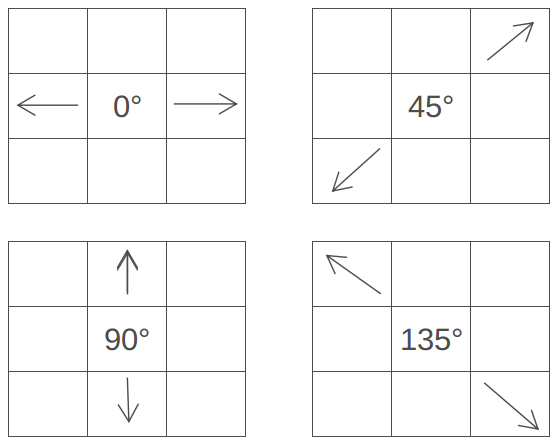
\includegraphics[scale=0.30]{./images/supression.png}
	\caption{Direcciones para realiza la supresi\'on de las magnitudes no-m\'aximas, esto para eliminar p\'ixeles que no son bordes.}
\end{figure}

Una caracter\'istica muy importante de este procedimiento es que como resultado se obtendr\'an unos bordes con un grosor de un pixel, lo que da una muy buena localizaci\'on de los bordes obtenidos, con respecto a los bordes reales.\\\\
Una vez que se eliminaron los p\'ixeles que no pueden considerarse bordes teniendo como par\'ametro de discriminaci\'on la magnitud de su gradiente, se procede al \'ultimo paso.

\textbf{\\ Hist\'eresis: \\\\}
Hasta el momento se tienen los bordes de una imagen con una muy buena localizaci\'on, pero a\'un existen bordes provenientes del ruido que es necesario eliminar y existen un conjunto de p\'ixeles no contiguos, los cuales pueden ser parte de un borde. Para ello es necesario realizar un seguimiento de dichos p\'ixeles para formar los bordes.\\

Al aplicar la hist\'eresis es necesario utilizar una doble umbralizaci\'on y, de acuerdo a los dos umbrales, se agrupan los p\'ixeles en tres categor\'ias: \\

\begin{itemize}
	\item \textbf{Fuertes}: son aquellos p\'ixeles cuyo valor es mayor o igual al umbral alto.
	\item \textbf{Medios}: se considera a aquellos p\'ixeles cuyo valor esta entre el umbra alto y el umbra bajo.
	\item \textbf{D\'ebiles}: son todos los p\'ixeles cuyo valor es menor o igual al umbra bajo.\\
\end{itemize}

Tomando como referencia la gr\'afica de la Figura 2., $T_1$ y $T_2$ son los umbrales bajo y alto respecticamente, a partir de estos dos umbrales comienza la categorizaci\'on de los p\'ixeles.\\

\begin{figure}[h]
	\setlength{\unitlength}{0.0125in}
	\centering
	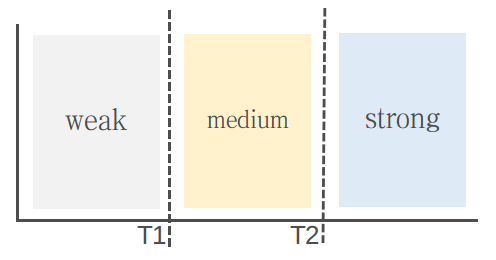
\includegraphics[scale=0.40]{./images/histeresis.png}
	\caption{Gr\'afica de la doble umbralizaci\'on y como deben separarse los p\'ixeles dependiendo de sus valores.}	
\end{figure}
\newpage
Una vez se tiene una categorizaci\'on de los p\'ixeles, el siguiente paso es eliminar aquellos p\'ixeles que sean ``d\'ebiles'', mantener los que son ``fuertes'' y, en el caso de que sean p\'ixeles ``medios'', se realiza el siguiente procedimiento:\\\\
Utilizando una ventana de 3x3 donde el pixel central es un pixel medio, se analiza si tiene al menos un vecino que sea ``fuerte'', para estos existen dos casos.\\
\begin{itemize}
	\item Se cuenta con al menos un pixel ``fuerte'' en el vecindaro: el pixel ``medio'' se vuelve ``fuerte''.
	\item No se tienen vecinos ``fuertes'': el pixel ``medio'' se elimina o se vuelve cero.\\
\end{itemize}

Para este paso es muy importante realizar los cambios en la misma imagen sobre la cual se est\'a haciendo el an\'alisis y categorizaci\'on de los p\'ixeles, esto para producir un seguimiento de los p\'ixeles que formar\'an los bordes.\\\\

\section{Resultados}
Para poder llevar a cabo las pruebas fue necesario elegir una imagen que tuviera una buena cantidad de bordes; los bordes se pueden encontrar en casas, ventanas, carros y objetos que est\'en conformados por figuras bien definidas como podr\'ian ser c\'irculos, cuadrados, rectangulos, tri\'angulos, etc.\\
La Figura 3., es una muestra de las im\'agenes que se utiliz\'o para realizar las pruebas.

\begin{figure}[h]
	\setlength{\unitlength}{0.115in}
	\centering
	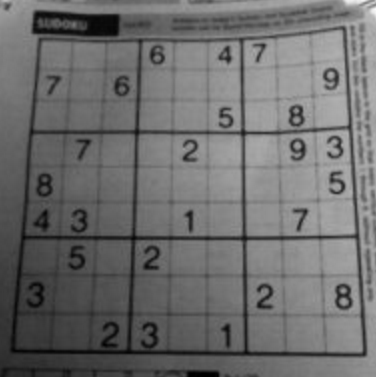
\includegraphics[scale=0.30]{./images/11sudoku.png}
	\caption{Foto de un SuDoKu, la cuale se utilizar\'a para probar la implementaci\'on del algoritmo de Canny.}
\end{figure}

\newpage
El primer paso de la implementaci\'on es hacer un suavizado en la imagen, el resultado de esta t\'ecnica se muestra en la Figura 4.

\begin{figure}[h]
	\setlength{\unitlength}{0.115in}
	\centering	
	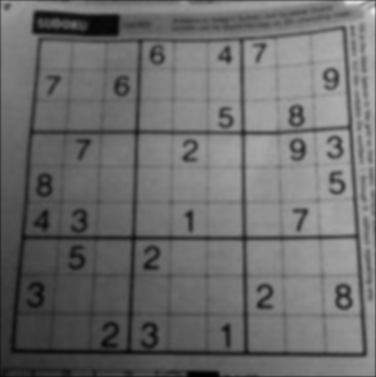
\includegraphics[scale=0.60]{./images/12sudokuBlur.png}
	\caption{Difuminado o suavizado que es el resultado de aplicar la Ecuaci\'on (2).}
\end{figure}
El paso anterior es simplemente para atenuar el ruido presente en la imagen ya que este se puede confundir como un bordes por el detector. Como se atenua y no se elimina completamente, pueden pasar p\'ixeles de ruido en el siguiente paso del algoritmo, para disminuirlo o eliminarlo se aplican otras t\'ecnicas.\\\\
Como siguiente paso se procede a obtener los bordes de la imagen, aplicando los kernel de convoluci\'on de la Ecuaci\'on (3), como resultado tenemos la imagen de la Figura 5.

\begin{figure}[h]
	\setlength{\unitlength}{0.105in}
	\centering
	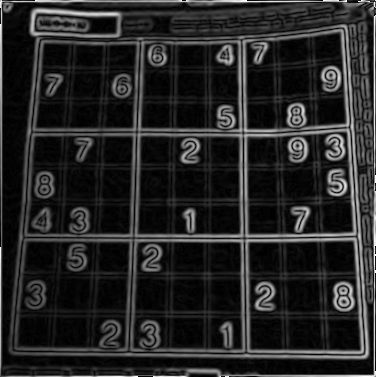
\includegraphics[scale=0.60]{./images/13sudokuEdges.png}
	\caption{Se obtienen el gradiente de la imagen con un filtro o kernel de primera derivada, las derivadas se realizan tanto en $x$ como en $y$.}
\end{figure}
En base al resultado se puede observar que los bordes mas dominantes se encuentran con un tono de gris mayor, que los bordes que no son dominantes. Este resultado es a causa de utilizar un filtro de derivada. Si, se obtienen los bordes analizando como $[-1, 1]$, como resultado tendr\'iamos unos bordes m\'as delgados lo cual es algo bueno, aunque el siguiente paso ser\'ia tambi\'en realiza lo mismo.\\\\

Una vez que se obtienen los bordes, el siguiente paso es la supresi\'on de los no-m\'aximos mostrado en la Figura 6.

\begin{figure}[h]
	\setlength{\unitlength}{0.105in}
	\centering	
	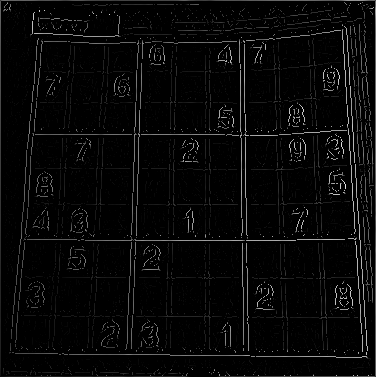
\includegraphics[scale=0.60]{./images/14sudokuSupression.png}
	\caption{Con la supresi\'on de los no-m\'aximos podemos eliminar los bordes que no tienen relevancia en la imagen y un poco de ruido.}
\end{figure}

Como resultado, los bordes se adelgazan a un grosor de un pixel, esto tambi\'en provoca que se diferencie a\'un m\'as entre los bordes con una mayor relevancia en la imagen que aquellos cuyor valor hace parecer como bordes ``d\'ebiles''.\\

El \'ultimo paso es aplicar la hist\'eresis sobre la imagen resultante de la supresi\'on de los p\'ixeles no-m\'aximos. Para realiza la hist\'eresis, se utilizan una doble umbralizaci\'on y, de acuerdo al valor de cada pixel y la secci\'on en la que se categoricen de acuerdo a la grafica de la Figura 2., se eliminan aquellos p\'ixeles ``d\'ebiles'' y los p\'ixeles ``medios'' que no tengan un pixel ``fuerte'' como vecino, esto a su vez, realiza un seguimiento para poder completar las lineas o bordes teniendo como resultado la imagen mostrada en la Figura 7.

\begin{figure}[h]
	\setlength{\unitlength}{0.105in}
	\centering
	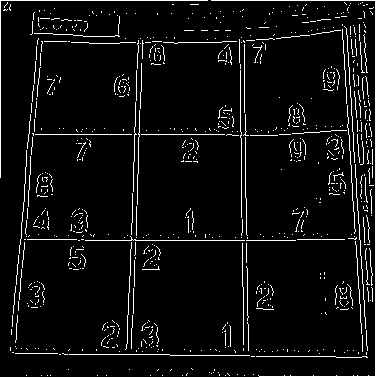
\includegraphics[scale=0.60]{./images/15sudokuHisteresis.png}
	\caption{Resultado de aplicar la hist\'eresis sobre la imagen.}
\end{figure}

\newpage
Cabe mencionar que la doble umbralizaci\'on se utiliza con un umbral alto y un umbral bajo. El valor del umbral bajo se tom\'o como $t_{1}=20$ y el umbral alto se calcula a partir del valor del umbral bajo, utilizando un ratio de $r=2$ o $r=3$, y se calcula como $highThreshold=lowThreshold*r$.\\\\

\section{Conclusiones}
El algoritmo de Canny es uno o posiblemente el mejor algoritmo para detectar los bordes de una imagen. Cada t\'ecnica o paso del algoritmo tiene un fundamento matem\'atico del porque se aplica y cual es el resultado esperado te\'orico, lo cual le agrega una robustez al algoritmo. Otra caracter\'istica importante es que es un algoritmo permite modificar par\'ametros en cada paso, esto da la oportunidad de agregar una matriz de convoluci\'on distinta en valores y dimensiones. Tambi\'en la posibilidad de modificar tanto el umbral bajo, ratio y, por ende, el umbral alto para adecuarlo a la imagen y sus propiedades.

%$\begin{bmatrix}
% 1 & 1 & 1 & 1 \\
% 1 & 1 & 1 & 1 \\
% 1 & 1 & 1 & 1 \\
% 1 & 1 & 1 & 1 \\
%\end{bmatrix}$

%\begin{thebibliography}{1}
%    \bibitem{IEEEhowto:kopka}
%    H.~Kopka and P.~W. Daly, \emph{A Guide to \LaTeX}, 3rd~ed.\hskip 1em plus
%      0.5em minus 0.4em\relax Harlow, England: Addison-Wesley, 1999.
%\end{thebibliography}

\end{document}
